\documentclass[12pt, a4paper]{article}
\usepackage[spanish]{babel}
\usepackage[utf8]{inputenc}
\usepackage{graphicx}
\usepackage{geometry}
\usepackage{fancyhdr}
\usepackage{float}
\usepackage{titling}

\geometry{a4paper, margin=2.5cm}
\pagestyle{fancy}
\fancyhf{}
\rhead{
\includegraphics[height=1.2cm]{images/logo-usm.png}} % Logo en encabezado
\lhead{Grupo 19\\Visualización de Datos}
\rfoot{Página \thepage}

% Configuración del logo en portada
\pretitle{
  \begin{center}
  \vspace{1cm}
  
\includegraphics[width=0.5\textwidth]{images/logo-usm.png}\\
  \vspace{1.5cm}
  \LARGE
}
\posttitle{\end{center}}

\title{Informe: Tecnología en la Vida Cotidiana}
\author{Felipe Campaña, Javier Gómez, Matias Elgueta}
\date{\today\\[2cm]
}

\begin{document}

\maketitle

\section*{Criterios de Selección}
\begin{itemize}
    \item Criterio 1: Porcentaje de uso de internet en el mundo
    \item Criterio 2: Porcentajes de contratacion de fibra en el mundo (top 10)
    \item Criterio 3: Horas en redes sociales por país
    \item Criterio 4: Evolución de clientes telecomunicación
    \item Criterio 5: **
    \item Criterio 6: **
\end{itemize}

\section*{Análisis Gráfico}

% Repite este bloque para cada gráfico (total 6)


% --------------------------------------------------------FC--------------------------------------------------
\subsubsection*{Integrante 1: Felipe Campaña}
Los criterios seleccionados por este integrante son los siguientes:
\begin{itemize}
    \item Criterio 1: Porcentaje de uso de internet en el mundo.
    \item Criterio 2: Porcentajes de contratación de fibra en el mundo (top 10).
\end{itemize}

\subsection{Justificación Contratación de Fibra Óptica Fija}

Este indicador representa cuántas personas por cada 100 habitantes tienen acceso a Internet mediante conexiones de alta velocidad y calidad, como la fibra óptica. Se seleccionó por las siguientes razones:

\begin{itemize}
    \item Permite evaluar el nivel de infraestructura tecnológica instalada en cada país.
    \item Refleja el grado de modernización digital real, más allá de la simple conexión.
    \item Está fuertemente asociado a la capacidad de ofrecer servicios avanzados, como streaming, teletrabajo o telecomunicaciones.
\end{itemize}

\subsection{Justificación Acceso a Internet en la Población}

Este indicador señala el porcentaje de personas que utilizan Internet, sin importar el tipo de conexión. Su elección se justificó por los siguientes motivos:

\begin{itemize}
    \item Entrega una visión más amplia e inclusiva del uso digital básico en cada país.
    \item Permite identificar regiones que aún enfrentan barreras de conectividad fundamentales.
    \item Refleja el impacto de políticas públicas, alfabetización digital y disponibilidad económica de servicios de conectividad.
\end{itemize}

\subsection*{Gráfico 1: Uso de internet de las personas en el mundo}
\begin{figure}[H]
    \centering
    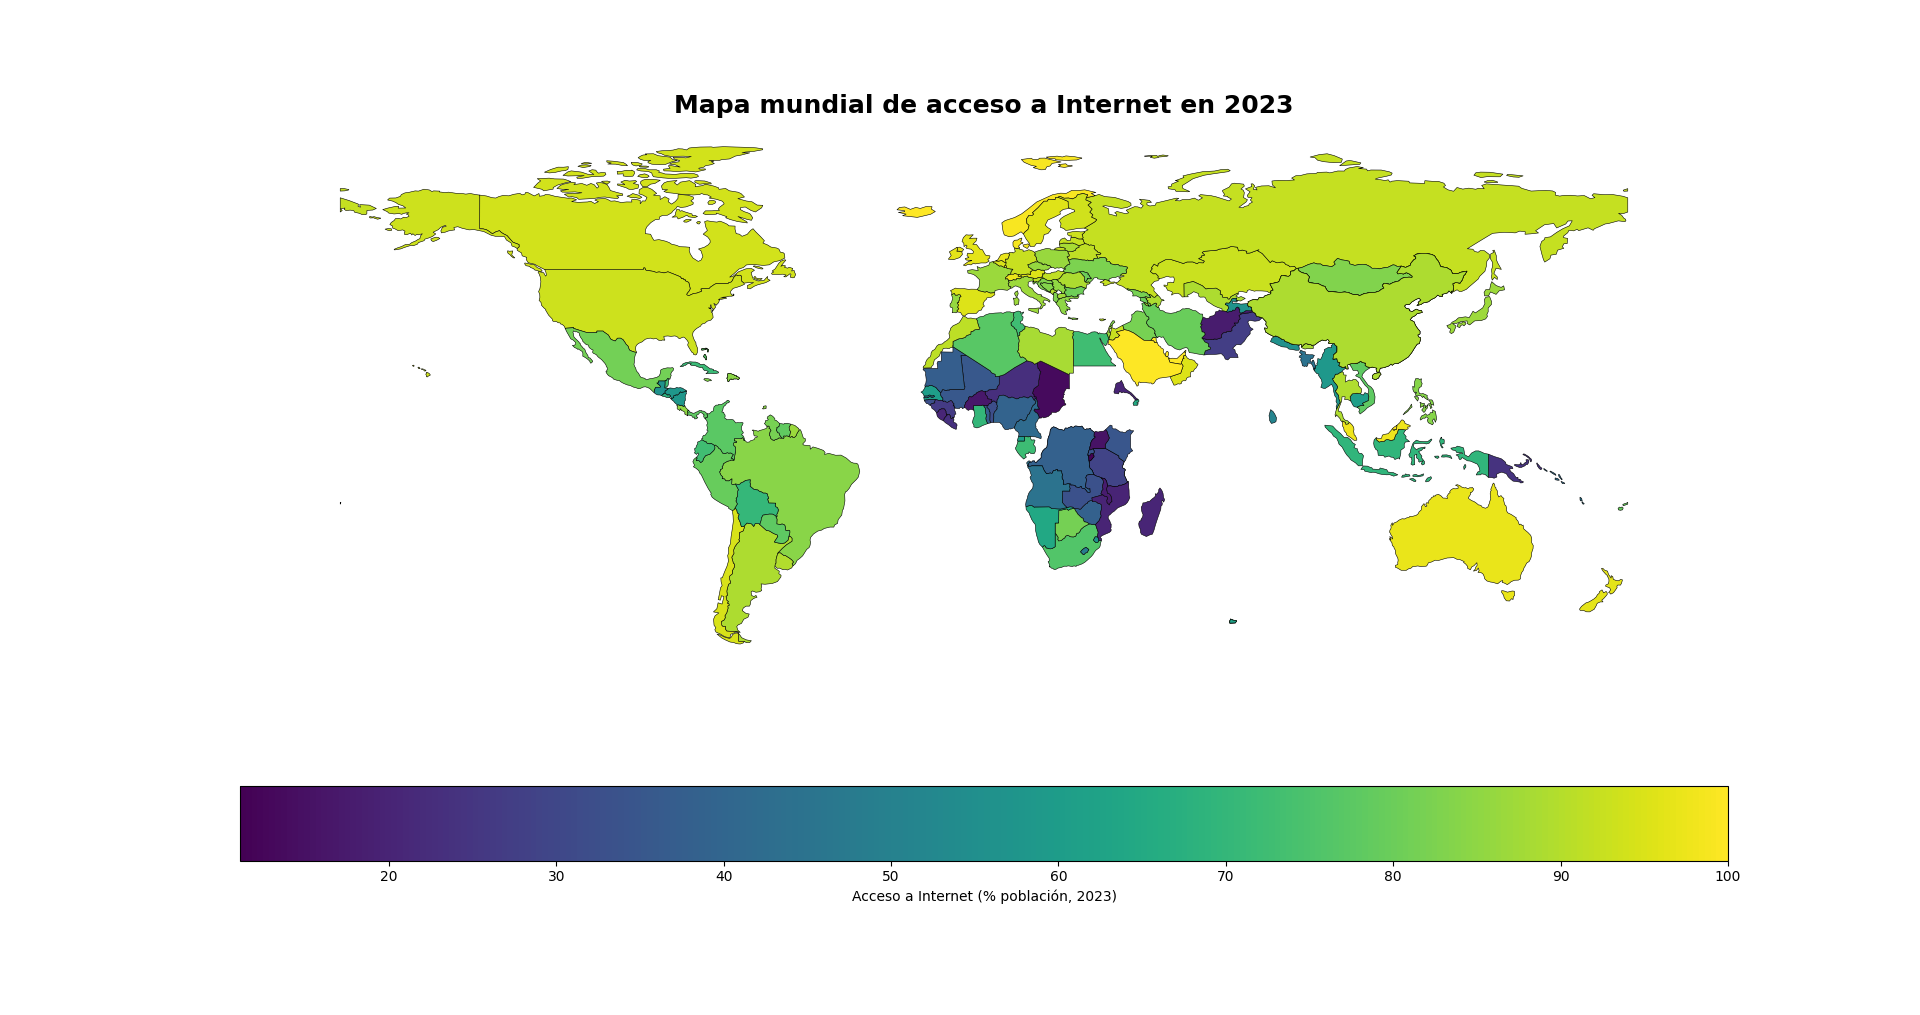
\includegraphics[width=0.85\textwidth]{images/Grafico_uso_de_internet_FC.png}
    \caption{Fuente: Elaboración propia con datos de [Worldbank], Link: [https://data.worldbank.org/indicator/IT.NET.USER.ZS?most_recent_value_desc=true&view=chart]}
\end{figure}

\subsubsection*{Conclusión}
\begin{itemize}
    \item Se observa que países como Mónaco (56\%), Andorra (52\%) y Liechtenstein (50\%) lideran la contratación de fibra en 2023.
    \item Son en general países pequeños, con economías desarrolladas y buena planificación urbana, lo que facilita la instalación de redes avanzadas.
    \item Países como China, Corea del Sur o Alemania también presentan cifras altas, pero no alcanzan el nivel de penetración de los primeros.
    \item El gráfico también muestra países con niveles más bajos, como Malta y Dinamarca (44\%), lo que sugiere diferencias internas incluso en regiones desarrolladas.
    \item Este tipo de visualización permite un contraste claro de adopción tecnológica y pone en evidencia el avance en infraestructura.
\end{itemize}

% Gráfico 2
\subsection*{Gráfico 2: Top 10 paises con mayor porcentaje de fibra contratada}
\begin{figure}[H]
    \centering
    \includegraphics[width=0.85\textwidth]{images/Grafico_fibra_contratada_FC.webp}
    \caption{Fuente: Elaboración propia con datos de [Worldbank], Link: [https://data.worldbank.org/indicator/IT.NET.BBND.P2]}
\end{figure}

\subsubsection*{Conclusión}
\begin{itemize}
    \item Muestra un panorama global del acceso digital: Europa, Oceanía y partes de Asia y América alcanzan más del 80\% de cobertura poblacional.
    \item África central y algunos países del sudeste asiático presentan niveles muy bajos (<40\%), lo que evidencia una brecha digital persistente.
    \item Países como Sudán, Congo o Yemen están en las zonas más oscuras del mapa, reflejando problemas estructurales en conectividad.
    \item Este mapa destaca diferencias regionales importantes que no necesariamente se reflejan en el gráfico de fibra óptica.
    \item Es una excelente forma de visualizar desigualdades sociales y tecnológicas a escala global.
\end{itemize}



% --------------------------------------------------------JG--------------------------------------------------
\subsection*{Gráfico 3: Aquí colocar título}
\begin{figure}[H]
    \centering
    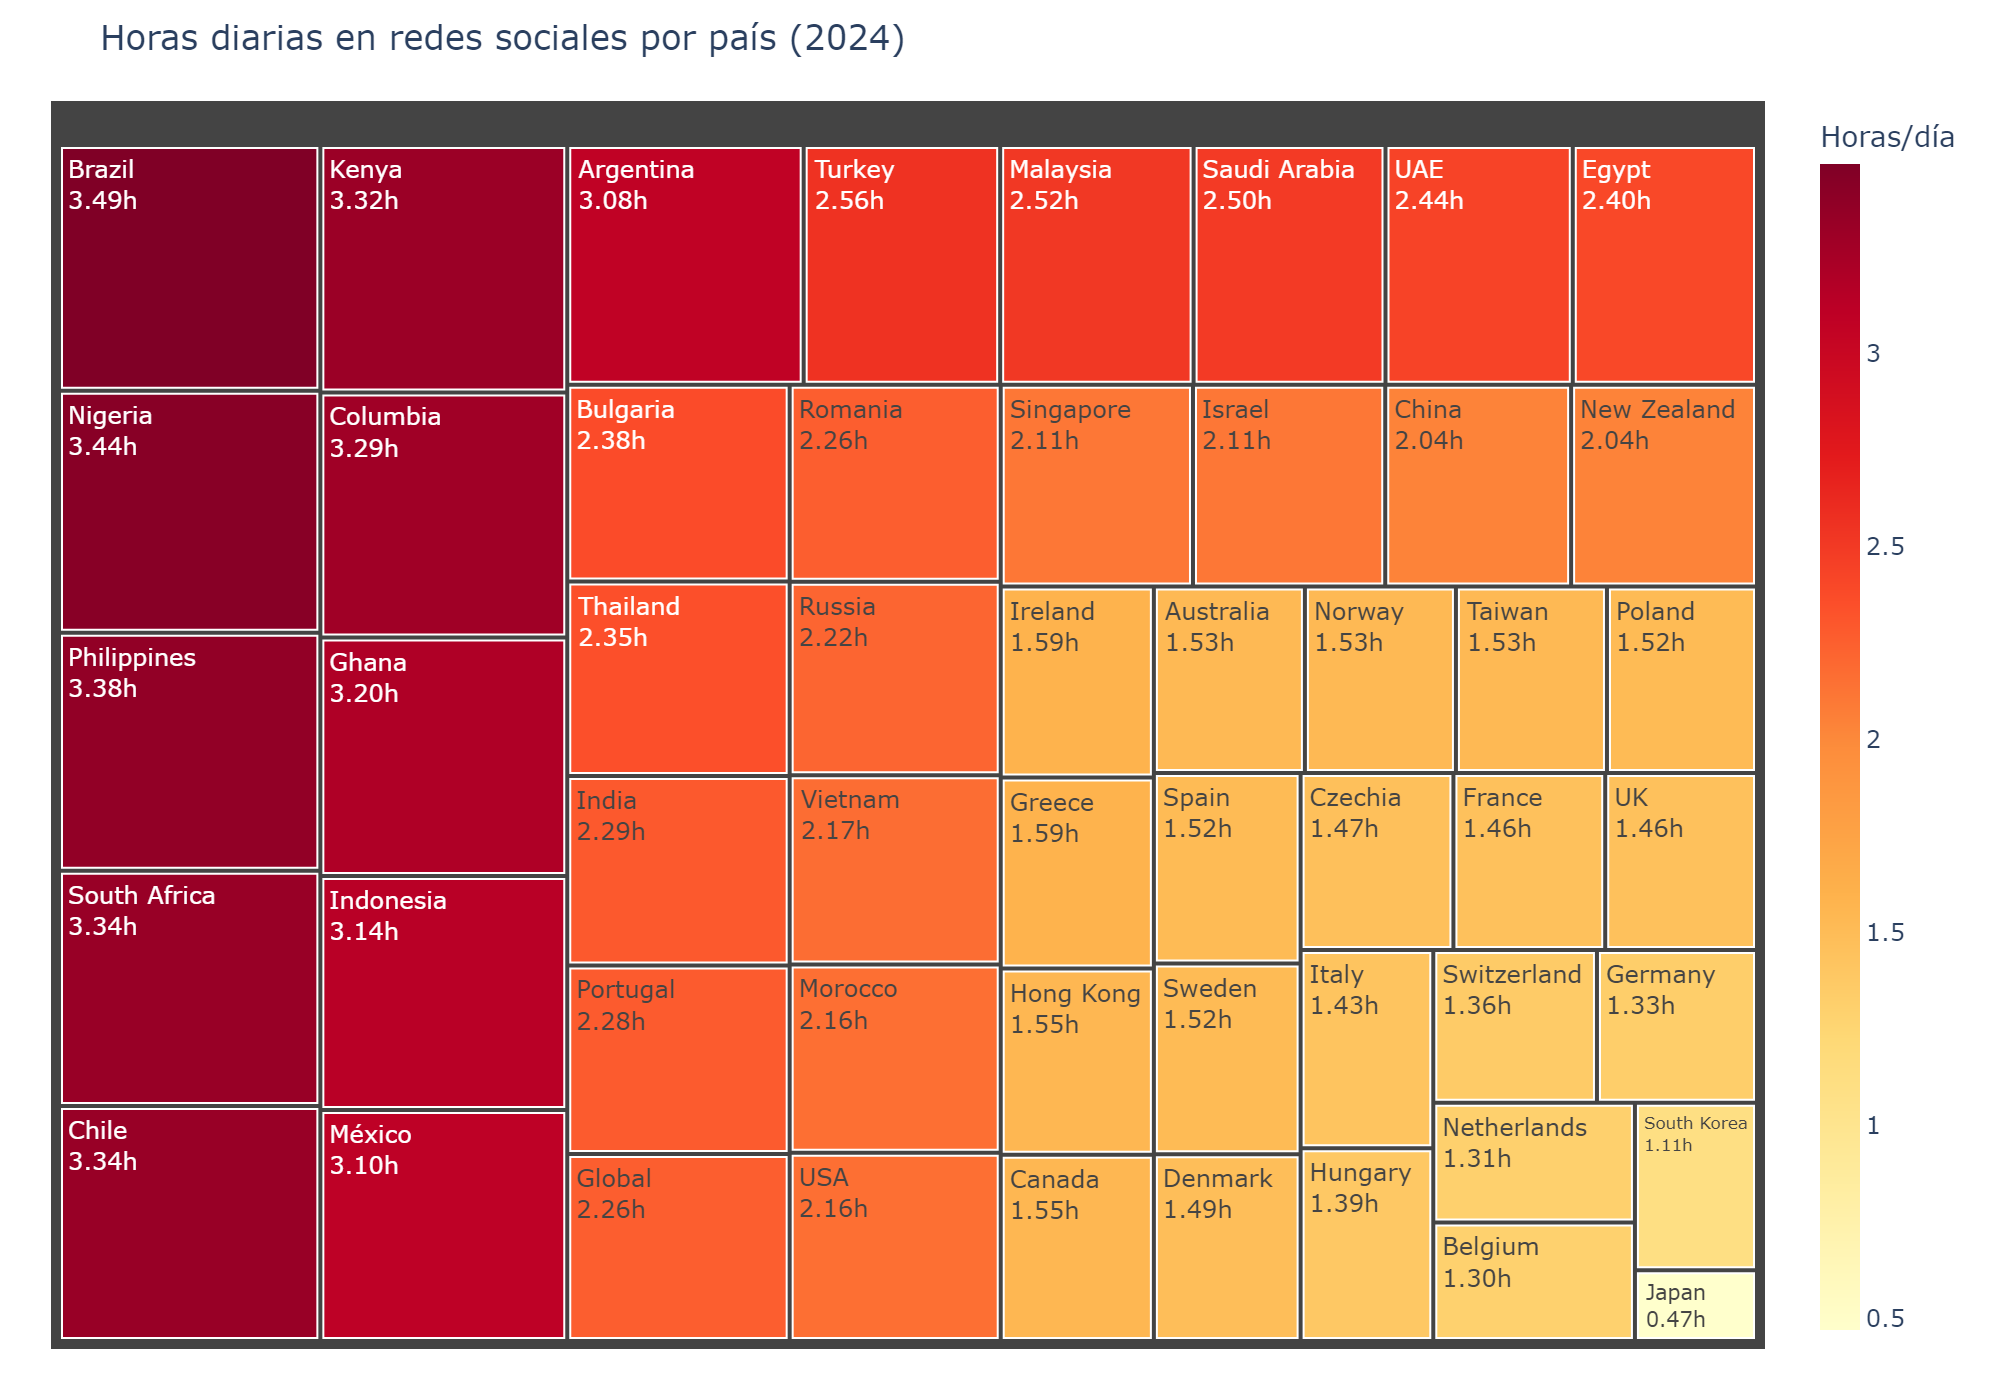
\includegraphics[width=0.85\textwidth]{images/graph1_JG.png}
    \caption{Fuente: Elaboración propia con datos de [Nombre de Fuente]}
\end{figure}

\subsubsection*{Conclusión}
Texto de conclusión específico para este gráfico. Analizar tendencias observadas y su relación con el impacto tecnológico en la vida cotidiana.

% Gráfico 2
\subsection*{Gráfico 4: Aquí colocar título}
\begin{figure}[H]
    \centering
    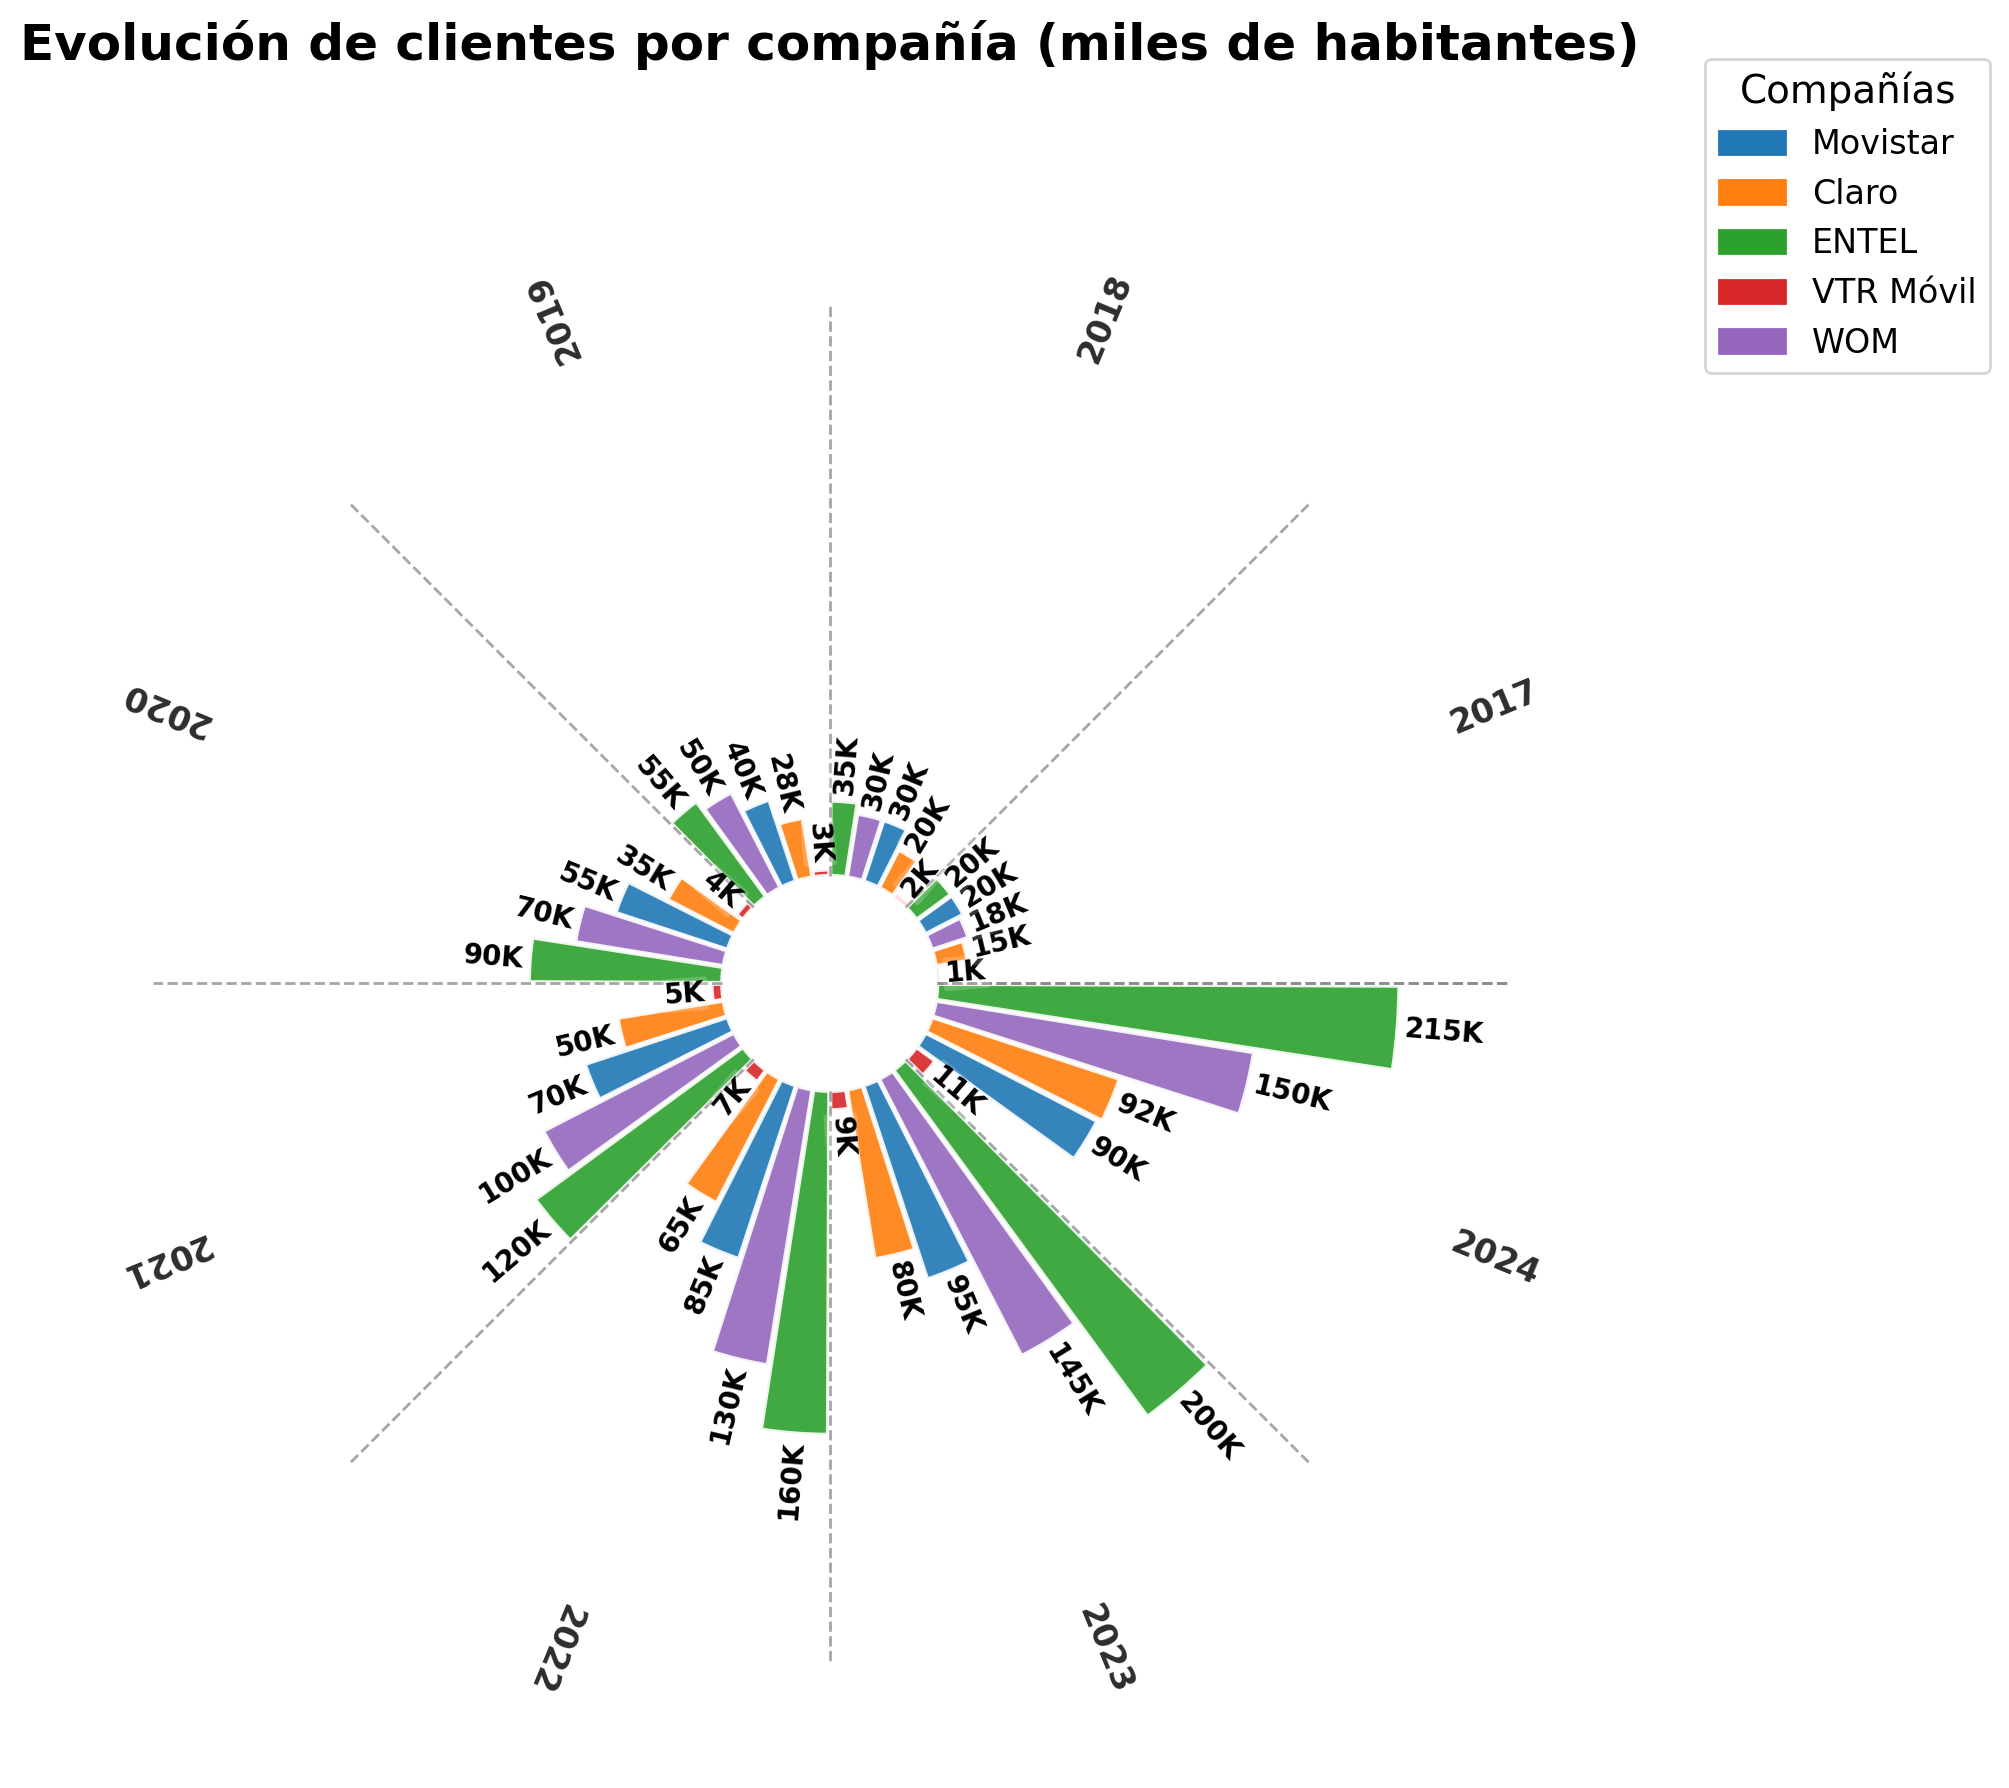
\includegraphics[width=0.85\textwidth]{images/graph2_JG.png}
    \caption{Fuente: Elaboración propia con datos de [Nombre de Fuente]}
\end{figure}

\subsubsection*{Conclusión}
Texto de conclusión específico para este gráfico. Analizar tendencias observadas y su relación con el impacto tecnológico en la vida cotidiana.

% Añadir los gráficos 3 al 6 siguiendo el mismo patrón

\section*{Conclusiones Generales}
\begin{itemize}
    \item Opcional**
  
\end{itemize}

\end{document}
